% IDS prvni cast


\documentclass[a4paper, 11pt]{article}
\usepackage[czech]{babel}
\usepackage[utf8]{inputenc}
\usepackage[left=2cm, top=3cm, text={17cm, 24cm}]{geometry}
\usepackage{times}
\usepackage{verbatim}
\usepackage{enumitem}
\usepackage{amsmath, bm}
\usepackage[graphicx]{realboxes}
\usepackage[unicode]{hyperref}
\usepackage{array, tabularx}
\usepackage{pdflscape}


\begin{document}


\begin{titlepage}
		\begin{center}
			
\includegraphics[width=0.85\linewidth]{./logo_cz.png} \\

			\vspace{\stretch{0.382}}

			\LARGE{Projekt 1. část} \\
			\Huge{\textbf{Model případů užití, ER diagram}} \\
            \bigskip
            \Large{\textbf{Kavárenský povaleč}} \\
            \Large{IDS \--\ Databázové systémy} \\
            
			\vspace{\stretch{0.6}}
		\end{center}

			\Large

   
            \begin{tabularx}{0.96\textwidth}{ll>{\raggedleft\arraybackslash}X}
                Marek Štěrba & \texttt{xsterb16} \\
                Jakub Gryc & \texttt{xgrycj03} &  \Large\today  \\
                 %&  &  & \\ 
                %\textbf{FUNEXP} & \ &  &  
			\end{tabularx}


        % \end{minipage}
	\end{titlepage}

\section{Zadání}
Představte si, že jste kavárenský povaleč, který tráví celé dny v~kavárnách po celém Brně,
a protože jste už vyzkoušeli spoustu kaváren a ne vždy vám v~každé kavárně káva chutnala,
rozhodli jste se vytvořit kavárenskou komunitu, ve které by si mohli lidé sdílet informace
o~brněnských kavárnách. Kavárny nabízejí kávy lišící se způsobem přípravy, chutí, kvalitou a oblastí původu.
Uživatel i zaměstnanec musí uvést své základní informace, uživatel nad to i údaje o~oblíbeném druhu
přípravy kávy (espresso, cappuccino, flat white, atd.), oblíbené kavárně, oblíbeném druhu
kávy a počtu vypitých káv denně, může psát recenze k~jednotlivým kavárnám, které navštívil.
Pokud se tak uživatel kávové komunity rozhodne navštívit nějakou kavárnu, může si díky kavárenské
komunitě zjistit informace o~tom, kde se kavárna nachází, jaké má otvírací hodiny, kapacitu míst
a~její popis a~informace o~jejích zaměstnancích. Dále si může uživatel vyhledat jednotlivé recenze
a podle toho se rozhodnout, zda kavárnu navštíví nebo nikoliv. V~případě návštěvy kavárny pak sám může
buď sepsat recenzi, ve~které uvede, jak se mu kavárna líbila, přidělí jí určitý počet hvězdiček a uvede,
kdy kavárnu navštívil, nebo může hodnotit recenze ostatních uživatelů. Na recenze mohou zaměstnanci kaváren reagovat,
aby se mohli ohradit vůči pomluvám, přičemž tyto reakce mohou být taktéž hodnoceny uživateli.
V~systému se uchová nejen datum, kdy byla recenze nebo reakce napsána, ale i počet palců nahoru nebo dolů,
kterými byly ohodnoceny.

\section{Diagram případů užití}

\begin{center}
			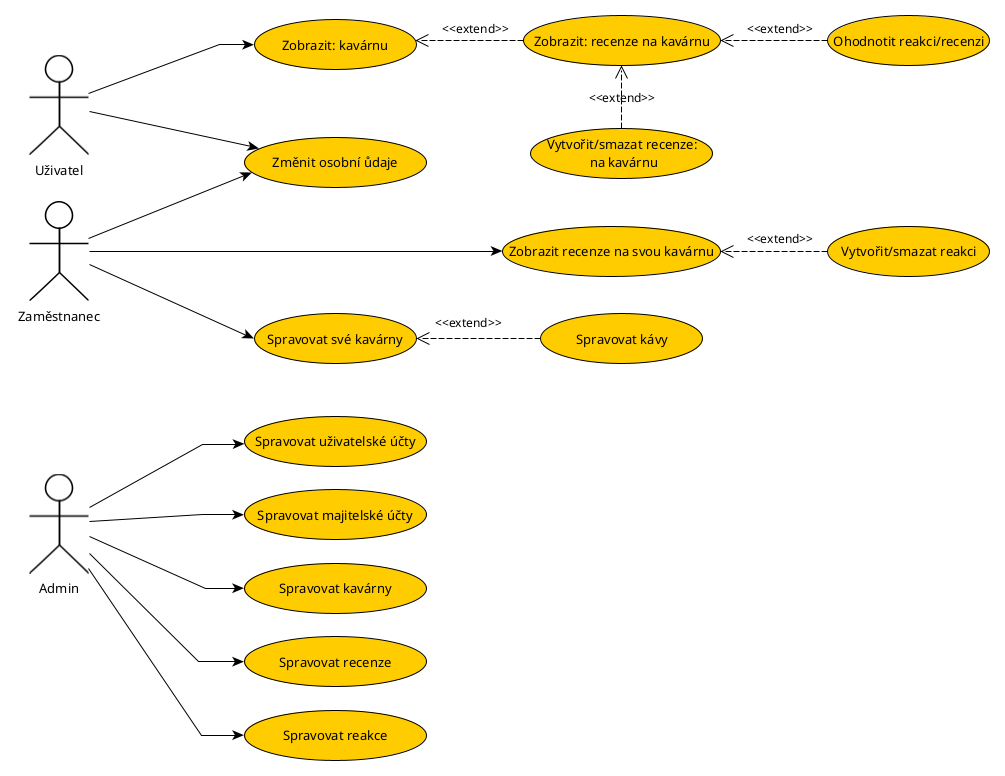
\includegraphics[width=1\linewidth]{./IDS_UCD.png} \\
            \label{UCD}
\end{center}

\newpage
\section{ER diagram}
\begin{center}
			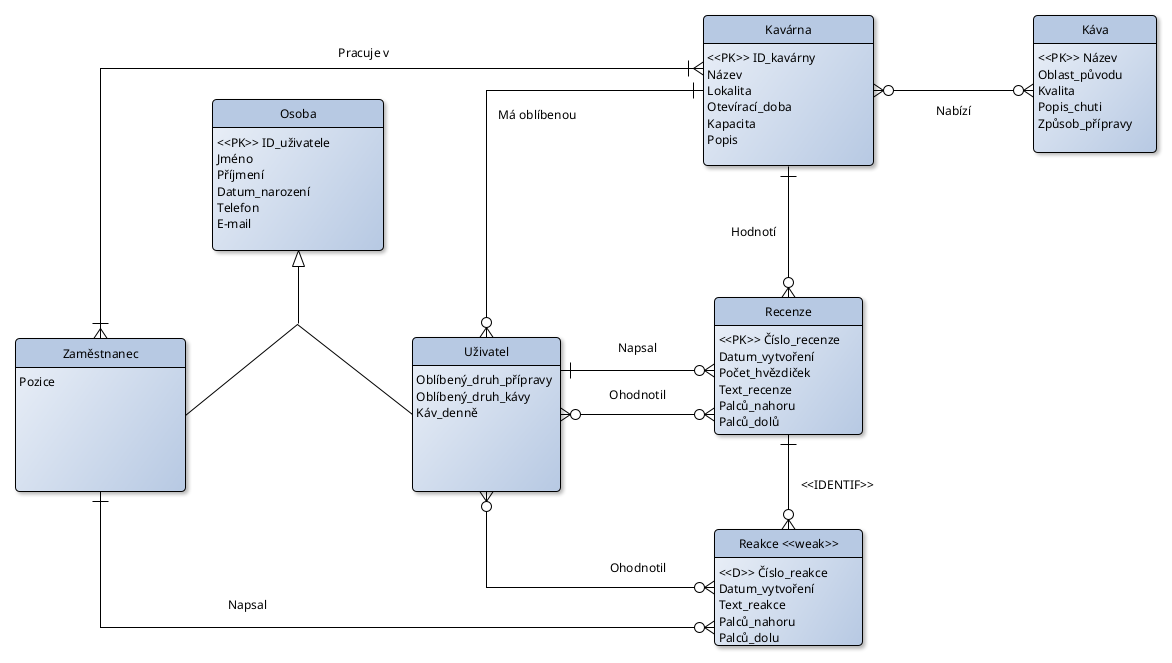
\includegraphics[width=1\linewidth]{./IDS_ER.png} \\
            \label{ER}
\end{center}
\end{document}
